\documentclass[t,handout]{beamer}

\usepackage[utf8]{inputenc}
\usepackage{minted}
\usepackage{tikz}

\title{Segment Trees}
\author{Aditya Arjun, Kevin Chen}
\institute{CS 104C}
\date{Fall 2019}

\setbeamertemplate{footline}[frame number]{}

\setbeamertemplate{navigation symbols}{}

\begin{document}
 
\frame{\titlepage}
 
\begin{frame}

    \frametitle{Computing Sums}

    \begin{itemize}
        \item \textbf{Problem: } Given an array $a$ which has $n$ integers. 
        
        \pause
        
        \item Given $q$ queries of the form $[l, r]$ (1-indexed, both inclusive).
        
        \pause
        
        \item For each query, return $a[l] + a[l + 1] + \cdots + a[r]$.
    \end{itemize}
    
    \pause
    
    \begin{itemize}
        \item Example: Say $a = [3, 5, 2, 7]$.
        
        \pause
        
        \item $(l, r) = (1, 4)$, then $sum = \pause 17$.
        
        \pause
        
        \item $(l, r) = (2, 3)$, then $sum = \pause 7$.
        
        \pause
        
        \item What's the overall runtime if we do this na\"ively over all queries?
        
        \pause
        
        \item $O(nq)$
    \end{itemize}

\end{frame}

\begin{frame}

    \frametitle{Prefix sums}

    \begin{itemize}

        \item

        Now we \textbf{precompute} some information that will help you answer queries faster. 
        
        \pause
        
        \item 
        
        $a = [3, 5, 2, 7]$
    
        \pause
        
        \item
        
        $p = [3, 8, 10, 17]$
        
        \pause
        
        \item 
        
        Given $p$, what is the formula for $\sum_{i = l}^r a[i]$ ?
        
        \pause
        
        \item
        
        $p[r] - p[l - 1]$ (assuming $l > 1$)
    \end{itemize}

\end{frame}

\begin{frame}

    \frametitle{Visualizing prefix sums}

    \begin{figure}
        \centering

        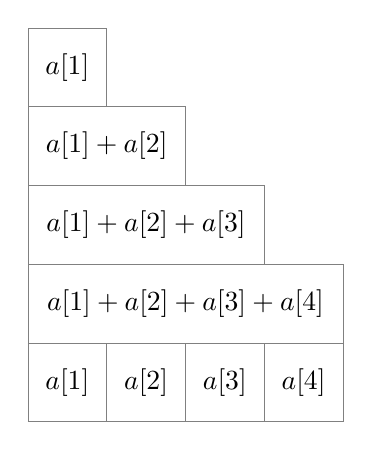
\begin{tikzpicture}
            \draw[step=1cm,gray,very thin] (0, 0) grid (4, 1);
            \draw[gray,very thin] (0, 1) rectangle (4, 2);
            \draw[gray,very thin] (0, 2) rectangle (3, 3);
            \draw[gray,very thin] (0, 3) rectangle (2, 4);
            \draw[gray,very thin] (0, 4) rectangle (1, 5);
            
            \node at (0.5, 0.5) {$a[1]$};
            \node at (1.5, 0.5) {$a[2]$};
            \node at (2.5, 0.5) {$a[3]$};
            \node at (3.5, 0.5) {$a[4]$};
        
           \node at (2, 1.5) {$a[1] + a[2] + a[3] + a[4]$};
            \node at (1.5, 2.5) {$a[1] + a[2] + a[3]$};
           \node at (1, 3.5) {$a[1] + a[2]$};
            \node at (0.5, 4.5) {$a[1]$};
        \end{tikzpicture}
    \end{figure}
\end{frame}

\begin{frame}

    \frametitle{Visualizing prefix sums}

    \begin{figure}
        \centering

        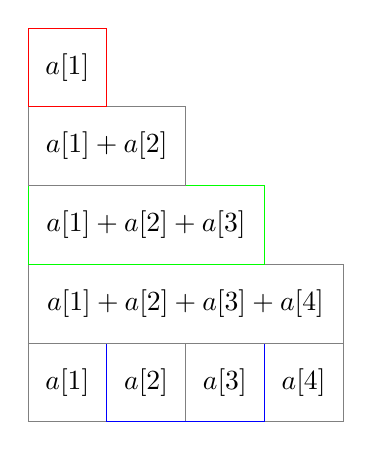
\begin{tikzpicture}
            \draw[step=1cm,gray,very thin] (0, 0) grid (4, 1);
            \draw[blue,very thin] (1, 0) rectangle (3, 1);
            
            \draw[gray,very thin] (0, 1) rectangle (4, 2);
            \draw[green,very thin] (0, 2) rectangle (3, 3);
            \draw[gray,very thin] (0, 3) rectangle (2, 4);
            \draw[red,very thin] (0, 4) rectangle (1, 5);
            
            \node at (0.5, 0.5) {$a[1]$};
            \node at (1.5, 0.5) {$a[2]$};
            \node at (2.5, 0.5) {$a[3]$};
            \node at (3.5, 0.5) {$a[4]$};
        
           \node at (2, 1.5) {$a[1] + a[2] + a[3] + a[4]$};
            \node at (1.5, 2.5) {$a[1] + a[2] + a[3]$};
           \node at (1, 3.5) {$a[1] + a[2]$};
            \node at (0.5, 4.5) {$a[1]$};
        \end{tikzpicture}
    \end{figure}
\end{frame}

\begin{frame}
    \frametitle{Prefix sum limitations}
    
    \begin{itemize}
        \item What functions can we use prefix sums on?
        
        \item We know addition and multiplication work 
        
        \pause
        
        \item The function needs to have an \emph{inverse}.
        
    \end{itemize}
\end{frame}

\begin{frame}

    \frametitle{Handling Updates}
    
    \begin{figure}
        \centering

        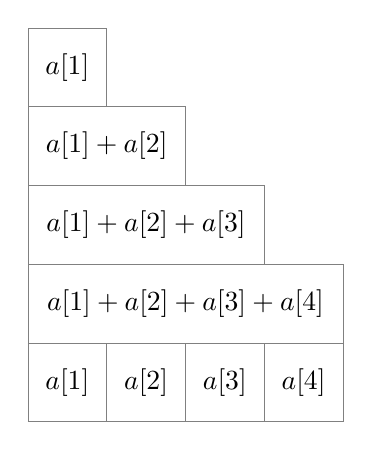
\begin{tikzpicture}
            \draw[step=1cm,gray,very thin] (0, 0) grid (4, 1);
            
            \draw[gray,very thin] (0, 1) rectangle (4, 2);
            \draw[gray,very thin] (0, 2) rectangle (3, 3);
            \draw[gray,very thin] (0, 3) rectangle (2, 4);
            \draw[gray,very thin] (0, 4) rectangle (1, 5);
            
            \node at (0.5, 0.5) {$a[1]$};
            \node at (1.5, 0.5) {$a[2]$};
            \node at (2.5, 0.5) {$a[3]$};
            \node at (3.5, 0.5) {$a[4]$};
        
           \node at (2, 1.5) {$a[1] + a[2] + a[3] + a[4]$};
            \node at (1.5, 2.5) {$a[1] + a[2] + a[3]$};
           \node at (1, 3.5) {$a[1] + a[2]$};
            \node at (0.5, 4.5) {$a[1]$};
        \end{tikzpicture}
    \end{figure}
    
    \begin{itemize}
        \item Say now we also allow updates to specific elements.
        
        \pause
        
        \item How many prefix sums do we need to update?
        
        \pause
        
        \item Each update requires changing $O(n)$ prefix sums.
        
        \pause
        
        \item Can we do better?
    \end{itemize}
\end{frame}

\begin{frame}

    \frametitle{Single block system}
    
    \begin{figure}
        \centering

        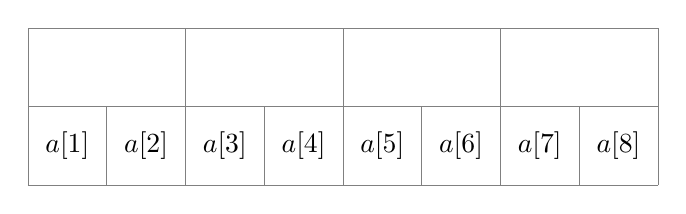
\begin{tikzpicture}
            \draw[step=2cm,gray,very thin] (0, 1) grid (8, 2);
            \draw[step=1cm,gray,very thin] (0, 0) grid (8, 1);
                        
            \node at (0.5, 0.5) {$a[1]$};
            \node at (1.5, 0.5) {$a[2]$};
            \node at (2.5, 0.5) {$a[3]$};
            \node at (3.5, 0.5) {$a[4]$};
            \node at (4.5, 0.5) {$a[5]$};
            \node at (5.5, 0.5) {$a[6]$};
            \node at (6.5, 0.5) {$a[7]$};
            \node at (7.5, 0.5) {$a[8]$};
        \end{tikzpicture}
    \end{figure}
    
    \begin{itemize}
        \item Say each element can only belong to a single block
        
        \pause
        
        \item What's the runtime for updating? \pause $O(1)$
        
        \pause
        
        \item What's the runtime to compute a sum? Let $B$ be the size of a block \pause $O(\max(B, N / B))$
        
        \pause
        
        \item What value of $B$ should we use to minimize the runtime? \pause $O(\sqrt{N})$.
        
        \pause
        
        \item This technique is called \textbf{Square Root decomposition}
    \end{itemize}
\end{frame}

\begin{frame}
    \frametitle{$O(\log(N))$ block system}
    
    \begin{figure}
        \centering

        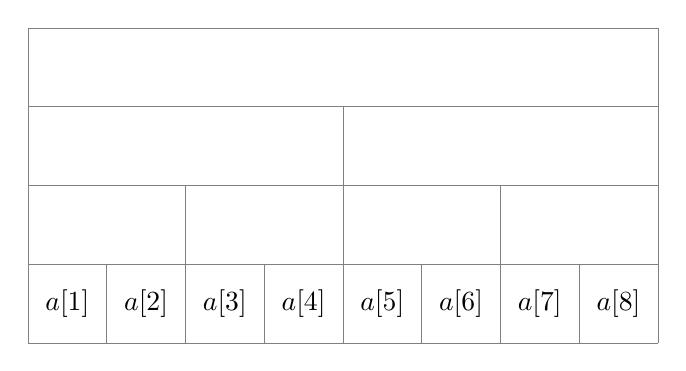
\begin{tikzpicture}
            \draw[step=8cm,gray,very thin] (0, 3) rectangle (8, 4);
            \draw[step=4cm,gray,very thin] (4, 2) rectangle (8, 3);
            \draw[step=4cm,gray,very thin] (0, 2) rectangle (4, 3);
            \draw[step=2cm,gray,very thin] (0, 1) grid (8, 2);
            \draw[step=1cm,gray,very thin] (0, 0) grid (8, 1);
                        
            \node at (0.5, 0.5) {$a[1]$};
            \node at (1.5, 0.5) {$a[2]$};
            \node at (2.5, 0.5) {$a[3]$};
            \node at (3.5, 0.5) {$a[4]$};
            \node at (4.5, 0.5) {$a[5]$};
            \node at (5.5, 0.5) {$a[6]$};
            \node at (6.5, 0.5) {$a[7]$};
            \node at (7.5, 0.5) {$a[8]$};
        \end{tikzpicture}
    \end{figure}
    
    \begin{itemize}
        \item Now let's allow each element to belong to $O(\log(N))$ blocks. 
        
        \item Each block is of size $2^k$.
        
        \pause
        
        \item What's the runtime for updating? \pause $O(\log(N))$
        
        \pause
        
        \item What's the runtime to compute a sum? \pause $O(\log(N))$
    \end{itemize}
\end{frame}

\begin{frame}
    \frametitle{Segment Trees}
    
    \begin{figure}
        \centering

        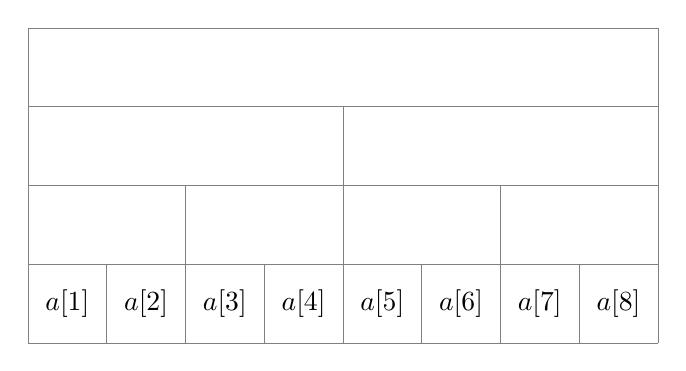
\begin{tikzpicture}
            \draw[step=8cm,gray,very thin] (0, 3) rectangle (8, 4);
            \draw[step=4cm,gray,very thin] (4, 2) rectangle (8, 3);
            \draw[step=4cm,gray,very thin] (0, 2) rectangle (4, 3);
            \draw[step=2cm,gray,very thin] (0, 1) grid (8, 2);
            \draw[step=1cm,gray,very thin] (0, 0) grid (8, 1);
                        
            \node at (0.5, 0.5) {$a[1]$};
            \node at (1.5, 0.5) {$a[2]$};
            \node at (2.5, 0.5) {$a[3]$};
            \node at (3.5, 0.5) {$a[4]$};
            \node at (4.5, 0.5) {$a[5]$};
            \node at (5.5, 0.5) {$a[6]$};
            \node at (6.5, 0.5) {$a[7]$};
            \node at (7.5, 0.5) {$a[8]$};
        \end{tikzpicture}
    \end{figure}
    
    \begin{itemize}
        \item The above structure is a binary tree called a \textbf{Segment Tree}.
    \end{itemize}
\end{frame}

\begin{frame}[fragile]
\frametitle{Implementation: Query}
\begin{itemize}
    \item Represent tree as an array; \texttt{tree[0]} is the root, and node $i$'s children are $2*i + 1$ and $2 * i + 2$.
    \item $i$ is the node in the tree
    \item $[l, r]$ is the interval that node $i$ contains the sum of.
    \item $[a, b]$ is the query interval.
    \item Returns the part of the interval sum contained in the subtree at node $i$
\end{itemize}
\begin{minted}{java}
    int[2 * N] tree;
    int query(int i, int l, int r, int a, int b) {
        if (r < a || l > b) return 0;
        if (l >= a || r <= b) return tree[i];
        return query(2 * i + 1, l, (l + r) / 2, a, b) +
            query(2 * i + 2, (l + r) / 2 + 1, r, a, b);
    }
\end{minted}
\pause
\begin{itemize}
    \item Why is the tree of size $2 * N$?
    \pause
    \item What if $N$ is not a power of 2?
\end{itemize}
\end{frame}

\begin{frame}[fragile]
\frametitle{Implementation: Update}
\begin{itemize}
    \item $i$ is the node in the tree
    \item $[l, r]$ is the interval that node $i$ contains the sum of.
    \item $j$ is the index we want to change.
    \item $v$ is the value we want to change $A[v]$ to.
    \item Recursive function returns value of \texttt{tree[i]} after applying \texttt{A[j] = v}
\end{itemize}
\begin{minted}{java}
    int update(int i, int l, int r, int v, int j) {
        if (j < l || j > r) return tree[i];
        if (l == r) {
            tree[i] = v
        } else {
            tree[i] =
                update(2 * i + 1, l, (l + r) / 2, j, v) +
                update(2 * i + 2, (l + r) / 2 + 1, r, j, v);
        };
        return tree[i];
    }
\end{minted}
\end{frame}

\begin{frame}
    \frametitle{Segment Tree Operations}
    
    \begin{itemize}
        \item What kinds of operations can be supported on a segment tree?
        
        \pause
        
        \item Any \textbf{associative} function will work
        
        \item Recall associative means $a + (b + c) = (a + b) + c$.
        
        \pause
        
        \item What are some examples of associative functions?
        
        \pause
        
        \item sum, product, min, max, gcd, matrix multiplication
        
        \pause
        
        \item What are not associative functions?
        
        \pause
        
        \item subtract, divide
    \end{itemize}
\end{frame}


\end{document}